\chapter{Návrh}

V této kapitole se budu věnovat návrhu knihovny na automatizaci a jejím funkčním požadavkům.

\section{Účastníci testování}
V rámci knihovny a testovacího běhu se bude vyskytovat několik účastníků testování. Mezi účastníky testování bude patřit:

\begin{description}
    \item[Testovací služba] Služba, která řídí testovací běh.
    \item[Testované zařízení] Hlavní účastník testování, který běží na jiném zařízení, než ze kterého běží testovací služba. 
    \item[Virtualizované zařízení] Zařízení, které simuluje nějakou činnost testovaného zařízení. Toto zařízení běží na stejném zařízení, jako testovací služba. 
\end{description}

Testovací služba bude jádrem k řízení testování. Tato služba poběží na samostatném zařízení. Toto zařízení bude běžet na operačním systému Windows. Zařízení bude v rámci infrastruktury serveru Azure DevOps agent. 

Hlavním cílem je testovat vyvíjený produkt. Toto zařízení v rámci knihovny bude bráno jako testované zařízení. Testovací služba bude podporovat připojení jednoho a více testovaných zařízení. Tato zařízení budou připojeno k zařízení, ze kterého poběží testovací služba, za pomocí Ethernet připojení. 

Součástí knihovny zároveň bude také tzv. virtualizované zařízení. Toto zařízení bude primárně sloužit k simulaci nějaké činnosti, kterou by jinak muselo provádět nějaké z testovaných zařízení. Simulováním testovaných zařízení snižujeme hardwarové nároky na testování, což vede ke snížení ekonomických nákladů na testování. Tato zařízení se budou připojovat v závislosti na jednotlivých testech. Následně po skončení testu budou tato zařízení odpojena.

\section{Komunikace}
Komunikace mezi všemi účastníky testování bude fungovat na principu TCP/IP připojení. Testovací služba a zařízení, na kterém služba poběží, bude sloužit jako server a všichni účastnící testovaní budou klienti, kteří se budou k tomuto zařízení připojovat. 

Jednotlivé zprávy, které budou mezi testovací službou a všemi účastníky testování vyměňovány, budou mít jasně stanovenou strukturu. Diagram složení zprávy lze vidět na obrázku \ref{fig:message}. Na tomto obrázku můžeme vidět, že jedna zpráva lze rozdělit na dvě části -- hlavičku zprávy a data zprávy. Zároveň jak můžeme vidět, jedna buňka v diagramu odpovídá jednomu bajtu. 

\begin{figure}[htbp]
    \centering 
    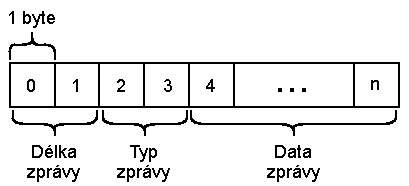
\includegraphics{assets/img/message.pdf}
    \caption{Diagram struktury jedné zprávy}
    \label{fig:message}
\end{figure}

Zpráva bude obsahovat povinně hlavičku zprávy. Tato hlavička bude obsahovat typ zprávy a délku dat zprávy. Jak můžeme vidět na diagramu, každý z těchto údajů bude mít velikost dva bajty. Celkově tedy hlavička bude o velikosti 4 bajty. Knihovna bude podporovat tyto typy zpráv:

\begin{enumerate}
    \item \inlinecode{MSG\_OK} -- Zpráva o úspěchu/potvrzení
    \item \inlinecode{MSG\_FAIL} -- Zpráva o neúspěchu
    \item \inlinecode{MSG\_TEST} -- Direktiva ke spuštění testu
    \item \inlinecode{MSG\_STOP} -- Direktiva k ukončení testování
\end{enumerate}

Za hlavičkou zprávy následně budou moct být uložena data zprávy. Tyto data avšak budou nepovinná. V těchto případech, kdy zpráva nebude neobsahovat data zprávy, bude pro přenesení informace postačovat pouze typ zprávy a v hlavičce bude uvedena nulová hodnota jako délka dat zprávy. 

Maximální délka jedné zprávy se bude odvíjet od limitací použitých technologií. Limit se bude primárně odvíjet od Ethernet protokolu, který podporuje nejmenší maximální délku jednoho packetu ze všech použitých protokolů, a to 1500 bajtů. Toto číslo avšak také zahrnuje všechny potřebné hlavičky k přenosu packetu. Proto jako maximální délka jedné zprávy bude zvolena délka 1400 bajtů. Toto číslo ponechává místo pro potřebné hlavičky a zároveň je více než dostatečné pro navrhované použití. \cite{max_packet_size} 

Všechny hodnoty zprávy budou ukládány v kladné (anglicky tzv. unsigned) podobě. Jedinou kontrolní informací, kterou bude zpráva obsahovat, je délka dat zprávy. Protokol TCP/IP avšak sám obsahuje jednoduchou detekci chyb. Všechny tyto kontroly budou považovány jako dostatečné.

Účastníci testování se na začátku připojí k testovací službě a odešlou inicializační zprávu. Tato zpráva bude typu 1 a v datech zprávy bude obsahovat svojí MAC adresu. Výjimkou budou virtualizované zařízení, která budou jako svoji MAC adresu odesílat adresu \inlinecode{DE:AD:BE:EF:00:00}. Díky tomu je testovací služba jednoduše identifikuje. Testovací služba následně odešle potvrzovací zprávu o úspěšném připojení s typem 1, bez žádných dat. V případě vzniku chyby služba odešle zprávu typu 2, bez dat. 

Pro započnutí testování a spuštění jednotlivých stádií testování služba odešle všem účastníkům testování zprávu s typem 3. V datech zprávy služba odesílá tyto data:

\begin{enumerate}
    \item Číselnou reprezentaci identifikátoru testu. Ten je uložen v prvních 4 bajtech dat zprávy.
    \item Číselnou reprezentaci identifikátoru, který určuje fázi testu. Uložen je ve dvou bajtech dat zprávy hned za identifikátorem testu. Fáze testování jsou blíže popsány v sekci \ref{test_run}.
\end{enumerate}

Služba následně čeká na odpověď od všech účastníků testování. Účastnící odesílají testovací službě po skončení testovacího stádia zprávu bez dat, s typem 1 v případě úspěchu a s typem 2 v případě neúspěchu. 

Po skončení testování služba odesílá všem účastníkům testování zprávu s typem 4, bez žádných dat. Ukázku komunikace můžeme vidět znázorněnou na sekvenčním diagramu, který je na obrázku \ref{fig:seqdiag}. Na tomto sekvenčním diagramu můžeme vidět výměnu zpráv mezi testovací službou a dvěma účastníky testování během úspěšného testovacího běhu. Direktiva \inlinecode{Message} znázorňuje jednu zprávu, kde v závorkách můžeme vidět nejdříve typ zprávy a následně data zprávy (pokud zpráva nějaká data obsahuje). V diagramu zároveň můžeme vidět cyklus, který reprezentuje spuštění všech testů.

\begin{figure}[htbp]
    \centering 
    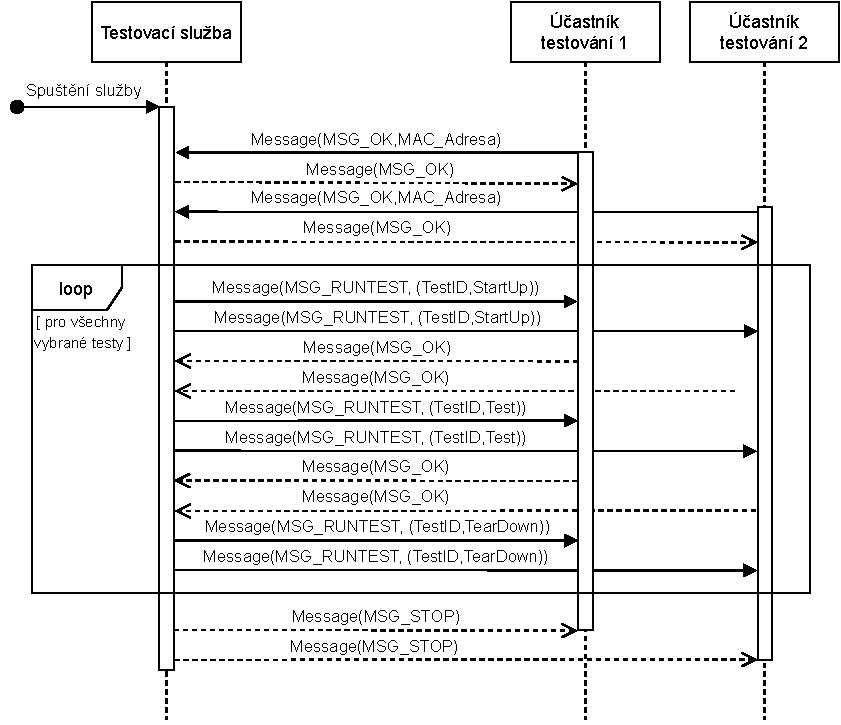
\includegraphics[width=0.95\textwidth]{assets/img/sequencediagram.pdf}
    \caption{Sekvenční diagram znázorňující běh služby}
    \label{fig:seqdiag}
\end{figure}

\section{Testovací služba}
Jak jsem již zmínil, testovací služba bude jádrem celého testování. Tato služba bude řídit celý testovací běh a předávat všem účastníkům testování pokyny. Zároveň bude synchronizovat testovací běh mezi všemi účastníky testování. 

\subsection{Inicializace služby}
Testovací služba započíná běh inicializační fází. Služba v inicializační fázi vytvoří připojení se všemi testovanými zařízeními, dle nadefinované komunikace. Z konfigurace služba bude vědět, kolik testovaných zařízení má očekávat. Inicializační fáze zároveň bude mít definovaný časový limit, který ve výchozí konfiguraci bude 60 sekund. Zároveň ale bude nastavitelný uživatelem. Testovací služba vyhodnotí inicializační fázi jako úspěšnou, pokud se úspěšně připojí definovaný počet testovaných zařízení. Služba vyhodnocuje neúspěch inicializační fáze v případě že nastanou tyto situace:

\begin{itemize}
    \item vypršení časového limitu na inicializační fázi
    \item chyba v komunikaci, nesprávná komunikace
    \item nepřipojení definovaného počtu zařízení
    \item připojení virtualizovaného zařízení
\end{itemize}

V případě neúspěchu inicializační fáze služba nastavuje stav služby jako chybný. Testy poté nebudou provedeny.

\subsection{Spravování virtualizovaných zařízení}
Jak již bylo nastíněno, služba bude podporovat připojení virtualizovaných zařízení. Tato zařízení se budou připojovat před spuštěním jednotlivých testů. Testovací služba obdrží direktivu k očekávaní připojení virtualizovaného zařízení. Toto zařízení projde stejnou inicializační fází jako ostatní testovaná zařízení. Služba vyhodnocuje neúspěch připojení virtualizovaného zařízení v těchto případech:

\begin{itemize}
    \item připojení jiného než virtualizovaného zařízení
    \item vypršení časového limitu na připojení
    \item chyba v komunikaci
\end{itemize}

V opačném případě služba vyhodnocuje úspěch. Po dokončení testu služba vysílá všem připojeným virtualizovaným zařízením direktivu k ukončení testování a ukončuje spojení s nimi.

\subsection{Testovací běh}\label{test_run}
Po úspěšné inicializační fázi a případném připojení virtualizovaných zařízení služba čeká na direktivu ke spuštění testu. Po obdržení této direktivy s identifikátorem testu služba odesílá všem účastníkům testování zprávu k zahájení první fáze testu. Tuto fázi budeme označovat jako přípravu na testování. V této fázi účastníci testovaní připraví všechny potřebné prostředky pro provedení testu. Účastníci následně odesílají zprávu o úspěchu/neúspěchu této fáze. Služba vyhodnocuje fázi jako úspěšnou pokud od všech účastníků obdrží zprávu o úspěchu. V opačném případě vyhodnocuje fázi jako neúspěšnou.

Služba po vyhodnocení úspěchu první fáze přechází do fáze druhé. V této fázi proběhne samotné testování. Služba odešle všem účastníkům zprávu ke spuštění této fáze. Následně očekává odpověď od všech účastníků. Služba, stejně jako v předchozí fázi, vyhodnocuje fázi jako úspěšnou, pokud obdrží zprávu o úspěchu od všech účastníků testování. V opačném případě je neúspěšná.

Poslední fází jednotlivého testu je úklid po testu. V této fázi služba opět vyšle zprávu k započetí fáze. Účastníci testování v této fázi uvádějí zařízení do stavu, ve kterém bylo před zahájením testu. Následně účastníci odešlou zprávu o úspěchu/neúspěchu. Vyhodnocení úspěchu/neúspěchu je stejné jako v předchozích fázích.

Po odeslání zprávy s direktivou k spuštění fáze testu služba čeká, než obdrží odpověď od všech účastníků testu. Tyto body, kdy služba čeká na odpověď od všech účastníků testu, budeme nazývat synchronizační body. Účastníci, kteří dokončili svojí fázi testu, čekají na direktivu od testovací služby. Tímto se běh synchronizuje mezi všemi účastníky testu. Jednoduše lze odvodit, že během jednoho testu nastávají tři synchronizační body. 

Tyto synchronizační body budou mít definovaný časový limit. Při spuštění testu tester bude moct zadat vlastní časový limit, který bude použit po každé z fází. Tedy tester bude zadávat předpokládaný maximální časový limit nejdelší fáze testování. Zároveň je ale potřeba vzít v úvahu, že časový limit je spuštěn ihned po odeslání všech zpráv. Tento časový limit bude ve výchozí konfiguraci opět 60 sekund. 

Testovaná zařízení se v době běhu testu mohou dostat do chybového stavu, ve kterém nebude možné pokračovat v testování. Testovací služba tedy bude předpokládat tyto chybné stavy:


\begin{description}
    \item[Nezajištění konzistence testování] Pro konzistenci testů testovací služba vyžaduje, aby po každém testu testované zařízení bylo ve stejném stavu jako bylo před začátkem testu. Pokud účastník testu odešle neúspěch ve fázi přípravy na test, nebo ve fázi úklidu po testu, tak poté bude tento účastník považován jako chybném stavu. V případě že chyba nastane ve fázi přípravy na test, služba neprovádí fázi testování a přechází do fáze úklidu po testu. 
    \item[Vypršení časového limitu] Vypršení časového limitu primárně znamená, že služba ve stanové době neobdržela odpověď od účastníka testování, ale tento účastník je stále připojen k testovací službě. Toto vede k závěru, že tento účastník je v chybovém stavu a další testování není možné. 
    \item[Chyba v komunikaci] Pokud během testu zařízení odpoví jinak, než dle stanovené komunikace, tak poté bude toto zařízení považováno jako v chybném stavu. Zároveň bude za chybu považováno odpojení zařízení od služby.  
\end{description}

Služba vyhodnocuje test jako úspěšný, pokud všechny fáze testu byli úspěšné. Obráceně služba vyhodnocuje test jako neúspěšný pokud jedna z fází byla neúspěšná. V případě nastání chyby, kde testované zařízení je předpokládáno jako v chybovém stavu, testovací služba nastavuje svůj stav jako chybový. Následující testy nebudou provedeny.


\subsection{Ukončení testování}
Testovací služba po obdržení direktivy k ukončení služby odesílá všem připojeným účastníkům testování zprávu k ukončení testovacího běhu. I když služba může některého z účastníků považovat jako v chybném stavu, pokud je tento účastník stále ke službě připojen, tak poté mu služba odešle tuto ukončovací zprávu. Toto se děje s cílem úspěšně ukončit co nejvíce zařízení.


\section{Rozhraní pro testování}
Důležitou součástí knihovny budou rozhraní, které umožní implementaci propojení s testovací službou a tím samotné testování. Knihovna bude obsahovat dvě důležitá rozhraní. 

\subsection{Rozhraní testu}
Jak jsem již popsal v sekci \ref{test_run}, jednotlivé testy budou mít tři fáze testování:

\begin{enumerate}
    \item Příprava na testování -- definování potřebných struktur, inicializace
    \item Testování -- provedení samotného testu
    \item Úklid po testu -- uvolnění využitých zdrojů
\end{enumerate}

Testovací knihovna tedy bude definovat rozhraní, které bude vyžadovat, aby tyto tři fáze testu byli pro každý test definované. Návrh rozhraní můžeme vidět na výpisu \ref{listing:test_if}. Na tomto výpisu můžeme vidět, že každé fázi odpovídá jedna metoda. Tyto metody následně vrací jednoduchou informaci o úspěchu/neúspěchu. To znamená, že vyhodnocení jednotlivých fází bude na jednotlivých testerech a jejich implementaci. Jednotlivé komponenty knihovny pouze obdrží informaci o výsledku fáze.

\begin{listing}[htbp]
    \begin{minted}[breaklines]{text}
    ITestCase 
    {
        bool StartUp()

        bool Test()

        bool TearDown()
    }
    \end{minted}
\caption{Návrh rozhraní pro jeden test}
\label{listing:test_if}
\end{listing}



\subsection{Rozhraní pro testované zařízení}

Dalším důležitým rozhraním bude rozhraní pro testované zařízení. Toto rozhraní bude definovat metody, které bude potřeba definovat na každém testovaném zařízení. Cílem je, aby toto rozhraní bylo co nejjednodušší pro co nejrychlejší implementaci na nově testovaném zařízení.

Návrh tohoto rozhraní můžeme vidět na výpisu \ref{listing:dev_if_abstract}. Jak můžeme z výpisu vidět vidět, první tři metody se starají o propojení s testovací službou. Metoda \inlinecode{createConnection} bude implementovat vytvoření propojení s testovací službou. Metoda pouze vytvoří propojení s testovací službou na základě TCP/IP protokolu a následně vrátí informaci o úspěšnosti. Cíl připojení, tedy IP adresu a port na kterém poběží testovací služba, metoda obdrží v argumentech.

O samotné odesílání, resp. přijímání jednotlivých zpráv se bude starat metoda \inlinecode{sendMessage}, resp. \inlinecode{rcvMessage}. Metoda \inlinecode{sendMessage} po svém zavolání převede objekt zprávy, obdržený v argumentu metody, na bajtové pole, které následně odešle testovací službě. Metoda \inlinecode{rcvMessage} symetricky zprávu od testovací služby přijme a převede ji na objekt jedné zprávy. Následně odkaz na tuto zprávu uloží do argumentu, který je výstupní. Obě tyto metody vrací informaci o úspěchu/neúspěchu.

Metoda \inlinecode{getTest} bude určena k získání jednotlivých instancí testů. Testy, které bude tato metoda vracet, musí být dle dříve zadefinovaného rozhraní pro jednotlivé testy. Metoda obdrží číselnou reprezentaci testu a na základě toho poté vrátí správnou instanci testu. 

Metoda \inlinecode{getMacAddress} bude, jak již z názvu vyplývá, vracet MAC adresu zařízení. V neposlední řadě metoda \inlinecode{print} bude sloužit k výpisu průběhu běhu. Tento výpis by měl hlavně posloužit k náhledu na průběh testovacího běhu, pokud se během běhu vyskytnou například nějaké chyby.

\begin{listing}[htbp]
    \begin{minted}[breaklines]{text}
    ITestClient 
    {

        bool createConnection(ipAddress, port)

        bool sendMessage(message)

        bool rcvMessage(message)

        ITestCase getTest(test)

        void print(toPrint)

        bool getMacAddress(macAddr)
    
    }
    \end{minted}
\caption{Ukázka definice rozhraní}
\label{listing:dev_if_abstract}
\end{listing}

\section{Běh testovaného zařízení}

O samotný běh jednotlivého testovaného zařízení se bude starat samostatná komponenta, která bude nezávislá na jakémkoliv zařízení. Tato komponenta se bude nazývat v knihovně tzv. \inlinecode{TestRunner}.

Komponenta bude obsahovat veškerou logiku testovacího běhu pro jednotlivé testované zařízení. Při zahájení testování komponenta za pomocí rozhraní vytvoří propojení s testovací službou a odešle zprávu o úspěchu, kde v datech zprávy uvede svoji MAC adresu. Po obdržení zprávy o úspěchu od testovací služby komponenta přechází do metody, která bude obsluhovat příchozí zprávy. 

Komponenta bude očekávat dva typy zpráv - direktivu ke spuštění testu a direktivu k ukončení testování. Po obdržení direktivy k započetí testu, komponenta ze zprávy zjistí identifikátor testu a testovací fázi. Následně z rozhraní získá instanci testu, který si po dobu běhu testu drží. Poté dle instrukcí spouští jednotlivé fáze testování. Po konci každé testovací fáze komponenta odesílá zprávu o úspěchu/neúspěchu testovací službě.

Dle této implementace může teoreticky dojít k tomu, že testované zařízení obdrží zprávu s požadavkem na spuštění fáze testování nebo fáze úklidu po testu, ještě předtím, než obdrží instrukci ke spuštění fáze přípravy na test. Komponenta tuto situaci kontroluje a v případě jejího vzniku automaticky odesílá zprávu o neúspěchu fáze. 

Průběh testovacího běhu testovaného zařízení lze vidět na diagramu aktivit, který můžeme vidět na obrázku \ref{fig:act_diag_device}. Jak lze z diagramu vidět, běh zařízení se silně odvíjí od příkazů, které obdrží od testovací služby. Zároveň na diagramu můžeme vidět již zmíněné tři synchronizační body. Tyto body jsou zvýrazněny modrým čárkovaným obdélníkem. Z diagramu se může zdát, že pokud zařízení ve fázi přípravy na testování nebo ve fázi úklidu po testu vrátí neúspěch, tak poté lze pokračovat v testování. Toto ale není pravda, protože tento případ testovací služba nepovolí a po dokončení tohoto testu, který způsobil danou chybu, bude testovací běh ukončen. Výjimkou jsou pouze virtualizované zařízení. Tyto zařízení jsou po konci testu ukončována, proto jejich chybný stav nemá následky na další testy.

\begin{figure}
    \centering 
    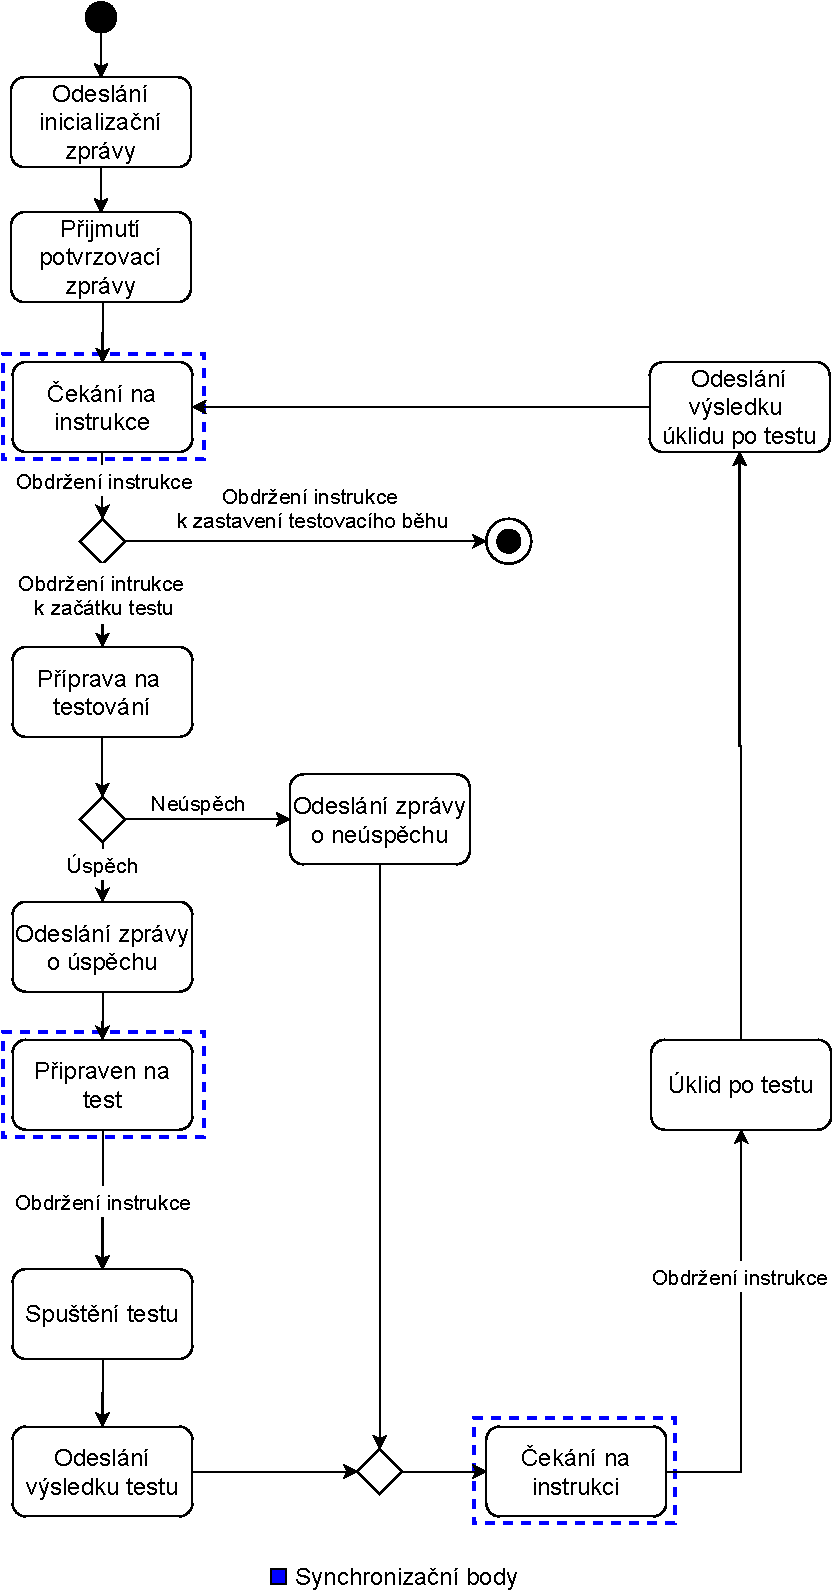
\includegraphics[height=0.98\textheight]{assets/img/activitydiagramdevice.pdf}
    \caption{Diagram aktivit testovaného zařízení}
    \label{fig:act_diag_device}
\end{figure}


\section{Virtualizované zařízení}
Virtualizované zařízení je speciálním druhem účastníka. Toto zařízení bude spouštěno ze stejného zařízení, jako testovací služba. Zařízení bude fungovat primárně na stejném principu, jako testovaná zařízení. Tedy, zařízení bude mít implementované rozhraní pro testované zařízení, které bude ovládáno komponentou \inlinecode{TestRunner}. 

Změnou je způsob ovládání této komponenty. Komponenta bude běžet ve vlastní třídě, která tuto komponentu bude spouštět na vlastním vlákně. Toto bude umožňovat nezávislý běh zařízení. Rozdílem také bude způsob definování testů. Virtualizované zařízení bude podporovat dva typy způsobů jak definovat testy. První způsobem bude za pomocí předání jedné instance testu. Jelikož virtualizované zařízení je vázáno na jednotlivé testy, je tento přístup nejjednodušší. Dalším způsobem bude předání funkce, která bude vracet instance testů na základě číselného identifikátoru. Tento způsob je totožný jako u testovaných zařízení a v určitých případech může usnadnit správu těchto zařízení. 

Tato zařízení, jak již bylo nastíněno, po konci testu budou odpojena od testovací služby. Zároveň bude kontrolováno jejich ukončení. V případě neúspěchu ukončení bude ukončeno vlákno, na kterém virtualizované zařízení poběží.

Testovací služba nebude nijak omezovat maximální možný počet připojených virtualizovaných zařízení. Jediné omezení, které teoreticky může vzniknout, bude v případě, že při vytváření vláken pro jednotlivá zařízení se vyčerpá maximální počet dostupných vláken. Toto by ale při reálném použití neměl být problém, jelikož je předpokládáno, že počet těchto zařízení využitých pro jeden test se bude pohybovat maximálně v desítkách. 

\section{Propojení se serverem Azure DevOps}
Jedním z cílů této práce je vytvoření takového připojení, aby server Azure DevOps byl schopen spouštět jednotlivé testy a zároveň obdržel výsledek testu. K tomuto propojení využijeme testovací framework MSTest. Vyvíjená testovací knihovna tedy poběží nad tímto testovacím frameworkem. Za pomoci frameworku MSTest bude server Azure DevOps schopen registrovat jednotlivé testy, a spouštět je jednotlivě.

\subsection{Propojení s frameworkem MSTest}
\todo{Doplnit}


\begin{figure}[htbp]
    \centering 
    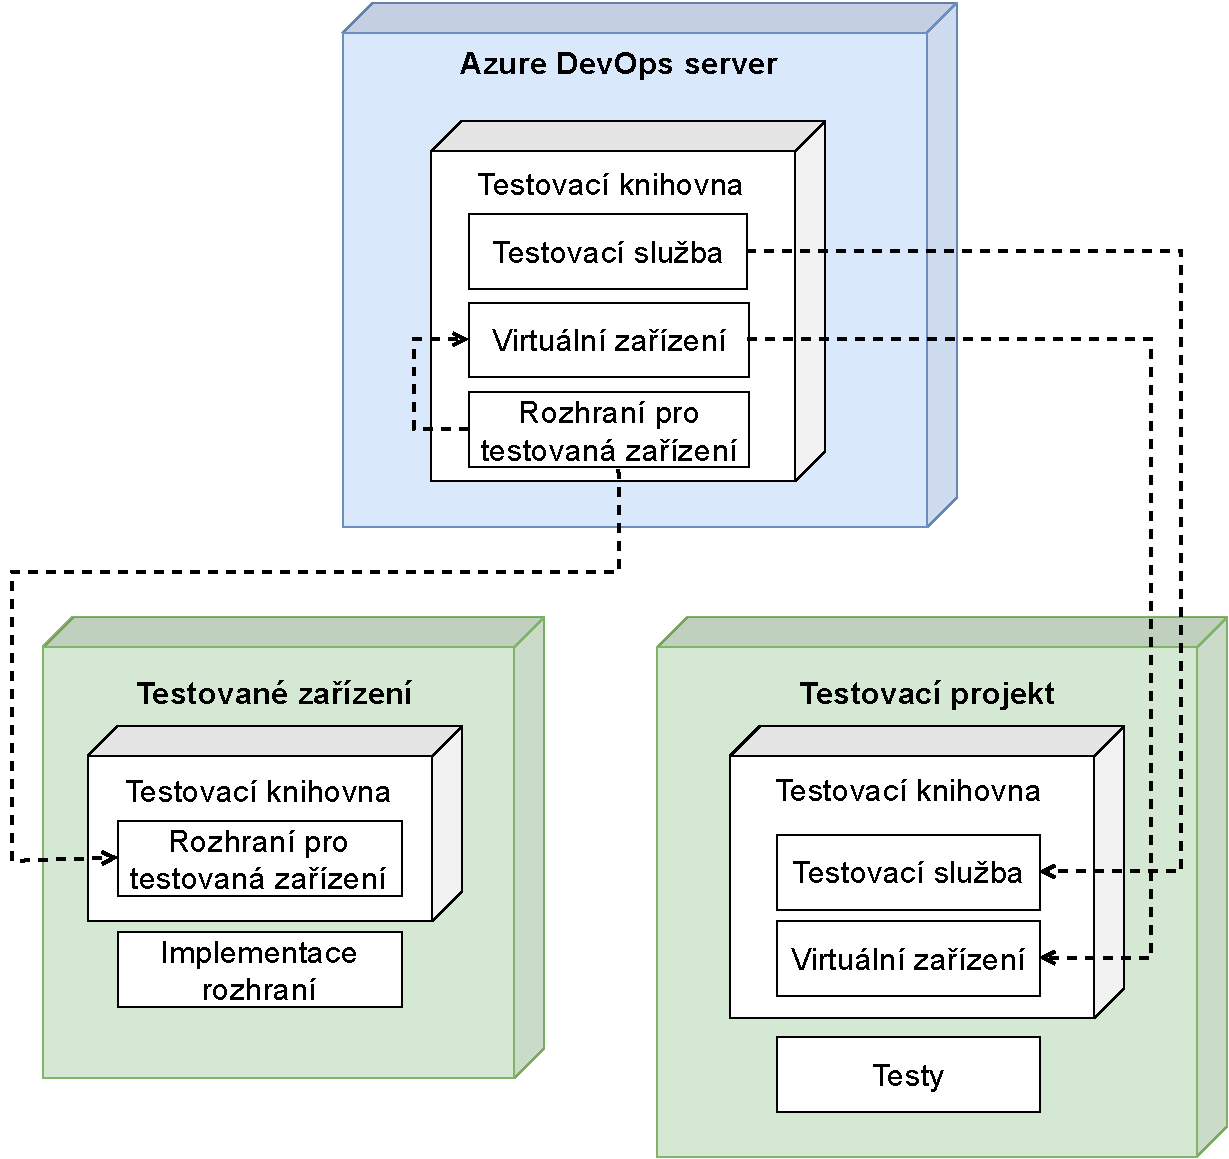
\includegraphics[width=0.95\textwidth]{assets/img/deploymentmodel.pdf}
    \caption{Deployment model}
    \label{fig:deploymodel}
\end{figure}